\chapter{Methodology} \label{CH:method}
%\textbf{How do you implement your Soln?\\
%Build a Fg HFM\\
%Use fgHFM to compute fgCurv\\
%Use fgCurv to infor cgCurv\\
%Use Curv's to solve RHS eqn\\
%Derive RHS eqn \& ref Herrmann as well as our modifications and $\delta$ approximation\\
%Use RHS to update fgVel\\
%Solve Poisson w/ new fgVel\\
%Fluxes happen somewhere in all of this???\\
%}\\

%This section will focus on the story of how the current model came to be. \\
%Start with the beginning: look on Box for presentations\\
%TIMELINE:\\
%
%
%Feb 2018 - PLIC reconstruction- area of discontinuity $\rightarrow$ velocity to drive back discontinuity\\
%Apr 2018 - velocity correction based on area times some factor $\rightarrow$ gives idea fro subgrid HFM\\
%May 2018- using matlab compute heights and curvature as 1/r \\
%Jun 2018 - Can show 5th order L2 error with mesh refinement (5th order finite difference scheme)\\
%Jul 2018 - ICLASS 2018 Poster - here we've tried several different discretization techniques\\
%Aug 2018 - Reintroduce SG velocity but allow to be influence by curvature rather than area\\
%Oct 2018 - Implement FG HFM but find parasitic wiggles $\rightarrow$ this is start of Herrmann correction and we add in 2nd pressure equation to ensure fine grid divergence free condition (12Oct18 presentation - late october is basically final APS presentation... same with november... thats the state at that point in time )\\
%Jan 2019 - Found discrepancy in Herrmann Eqn \\
%Mar 2019 - delta approximation big parametric study \\
%Apr 2019 - still doing para study \\

%Method development which would include information from the fine grid to reduce interface reconstruction discontinuities. 
%
%Introducing a fine grid velocity 

%With the standard implementation of NGA, VOF is calculated on the fine grid and curvature is computed on the coarse grid. 
%
%
%
%\begin{figure}[htbp]
%	\centering
%	\begin{tikzpicture}[scale=1.5]
%	% PLIC
%	\draw [lightblue,fill=lightblue] (0,0) -- (0,0.7) -- (1,0.7) -- (1,1.3) -- (2,1.3) -- (2,0) -- cycle;	
%	% VOF
%	\node at (0.5,0.5) {0.7};
%	\node at (1.5,0.5) {1};
%	\node at (0.5,1.5) {0};
%	\node at (1.5,1.5) {0.3};
%	%Cell
%	\draw [black, very thick] (0,0) -- (2,0) -- (2,2) -- (0,2) -- (0,0);
%	% Grid
%	\draw [blue, thick, dashed] (1,0) -- (1,2);
%	\draw [blue, thick, dashed] (0,1) -- (2,1);
%	\draw [arrows=->,line width=1.0] (0.5,0.7) -- (0.5,1.3);\node [left] at (0.49,1.1) {\scriptsize $v$};
%	\draw [arrows=->,line width=1.0] (1.7,1.7) -- (1.7,1.3);\node [right] at (1.705,1.5) {\scriptsize $v$};
%	\end{tikzpicture}
%	\caption{Advection of a one-dimensional fluid interface}
%	\label{fig:1Dadvect}
%\end{figure}

\subsection{Oscillating Droplet Test Case}
To further quantify the problem that is occurring, a baseline test case which highlights the shortcomings of current methods is necessary. To this end, an oscillating two-dimensional droplet is used to assess the height function method and the proposed solution methods. This test case was chosen as it is considered a standard benchmark problem for testing the accurate prediction of multiphase flow behavior\cite{Salih2002}. Additionally, for the height function method, the oscillating droplet offers an extensive testing of interface orientations which is important for measuring the robustness of the method. The interface is initialized with an ellipsoid. Surface tension drives the droplet's semi-major axis to fluctuate between alignment with the $x$ and $y$ axes. The period of oscillation $T_{e}$, is a function of surface tension coefficient ($\sigma$), density ($\rho_l$ and $\rho_g$), and equivalent circular radius($R$), and can be computed analytically as~\cite{Rayleigh}
\begin{equation}
T_{e} = 2 \pi \sqrt{\frac{(\rho_{l}+\rho_{g})R^3}{6\sigma}}.
\label{period}
\end{equation}

To establish successful oscillating droplet performance, an alternate curvature scheme was used and the simulation was run. Figure \ref{fig:acesKE} shows kinetic energy conservation through the progression of the simulation. Simulation success is quantified by normal periods of oscillation and diminishing kinetic energy with time. Close adherence to this model can be used as a measure of success with cases from here forward and this case will be plotted with all further test cases. 

\begin{figure}[h]
	\centering
	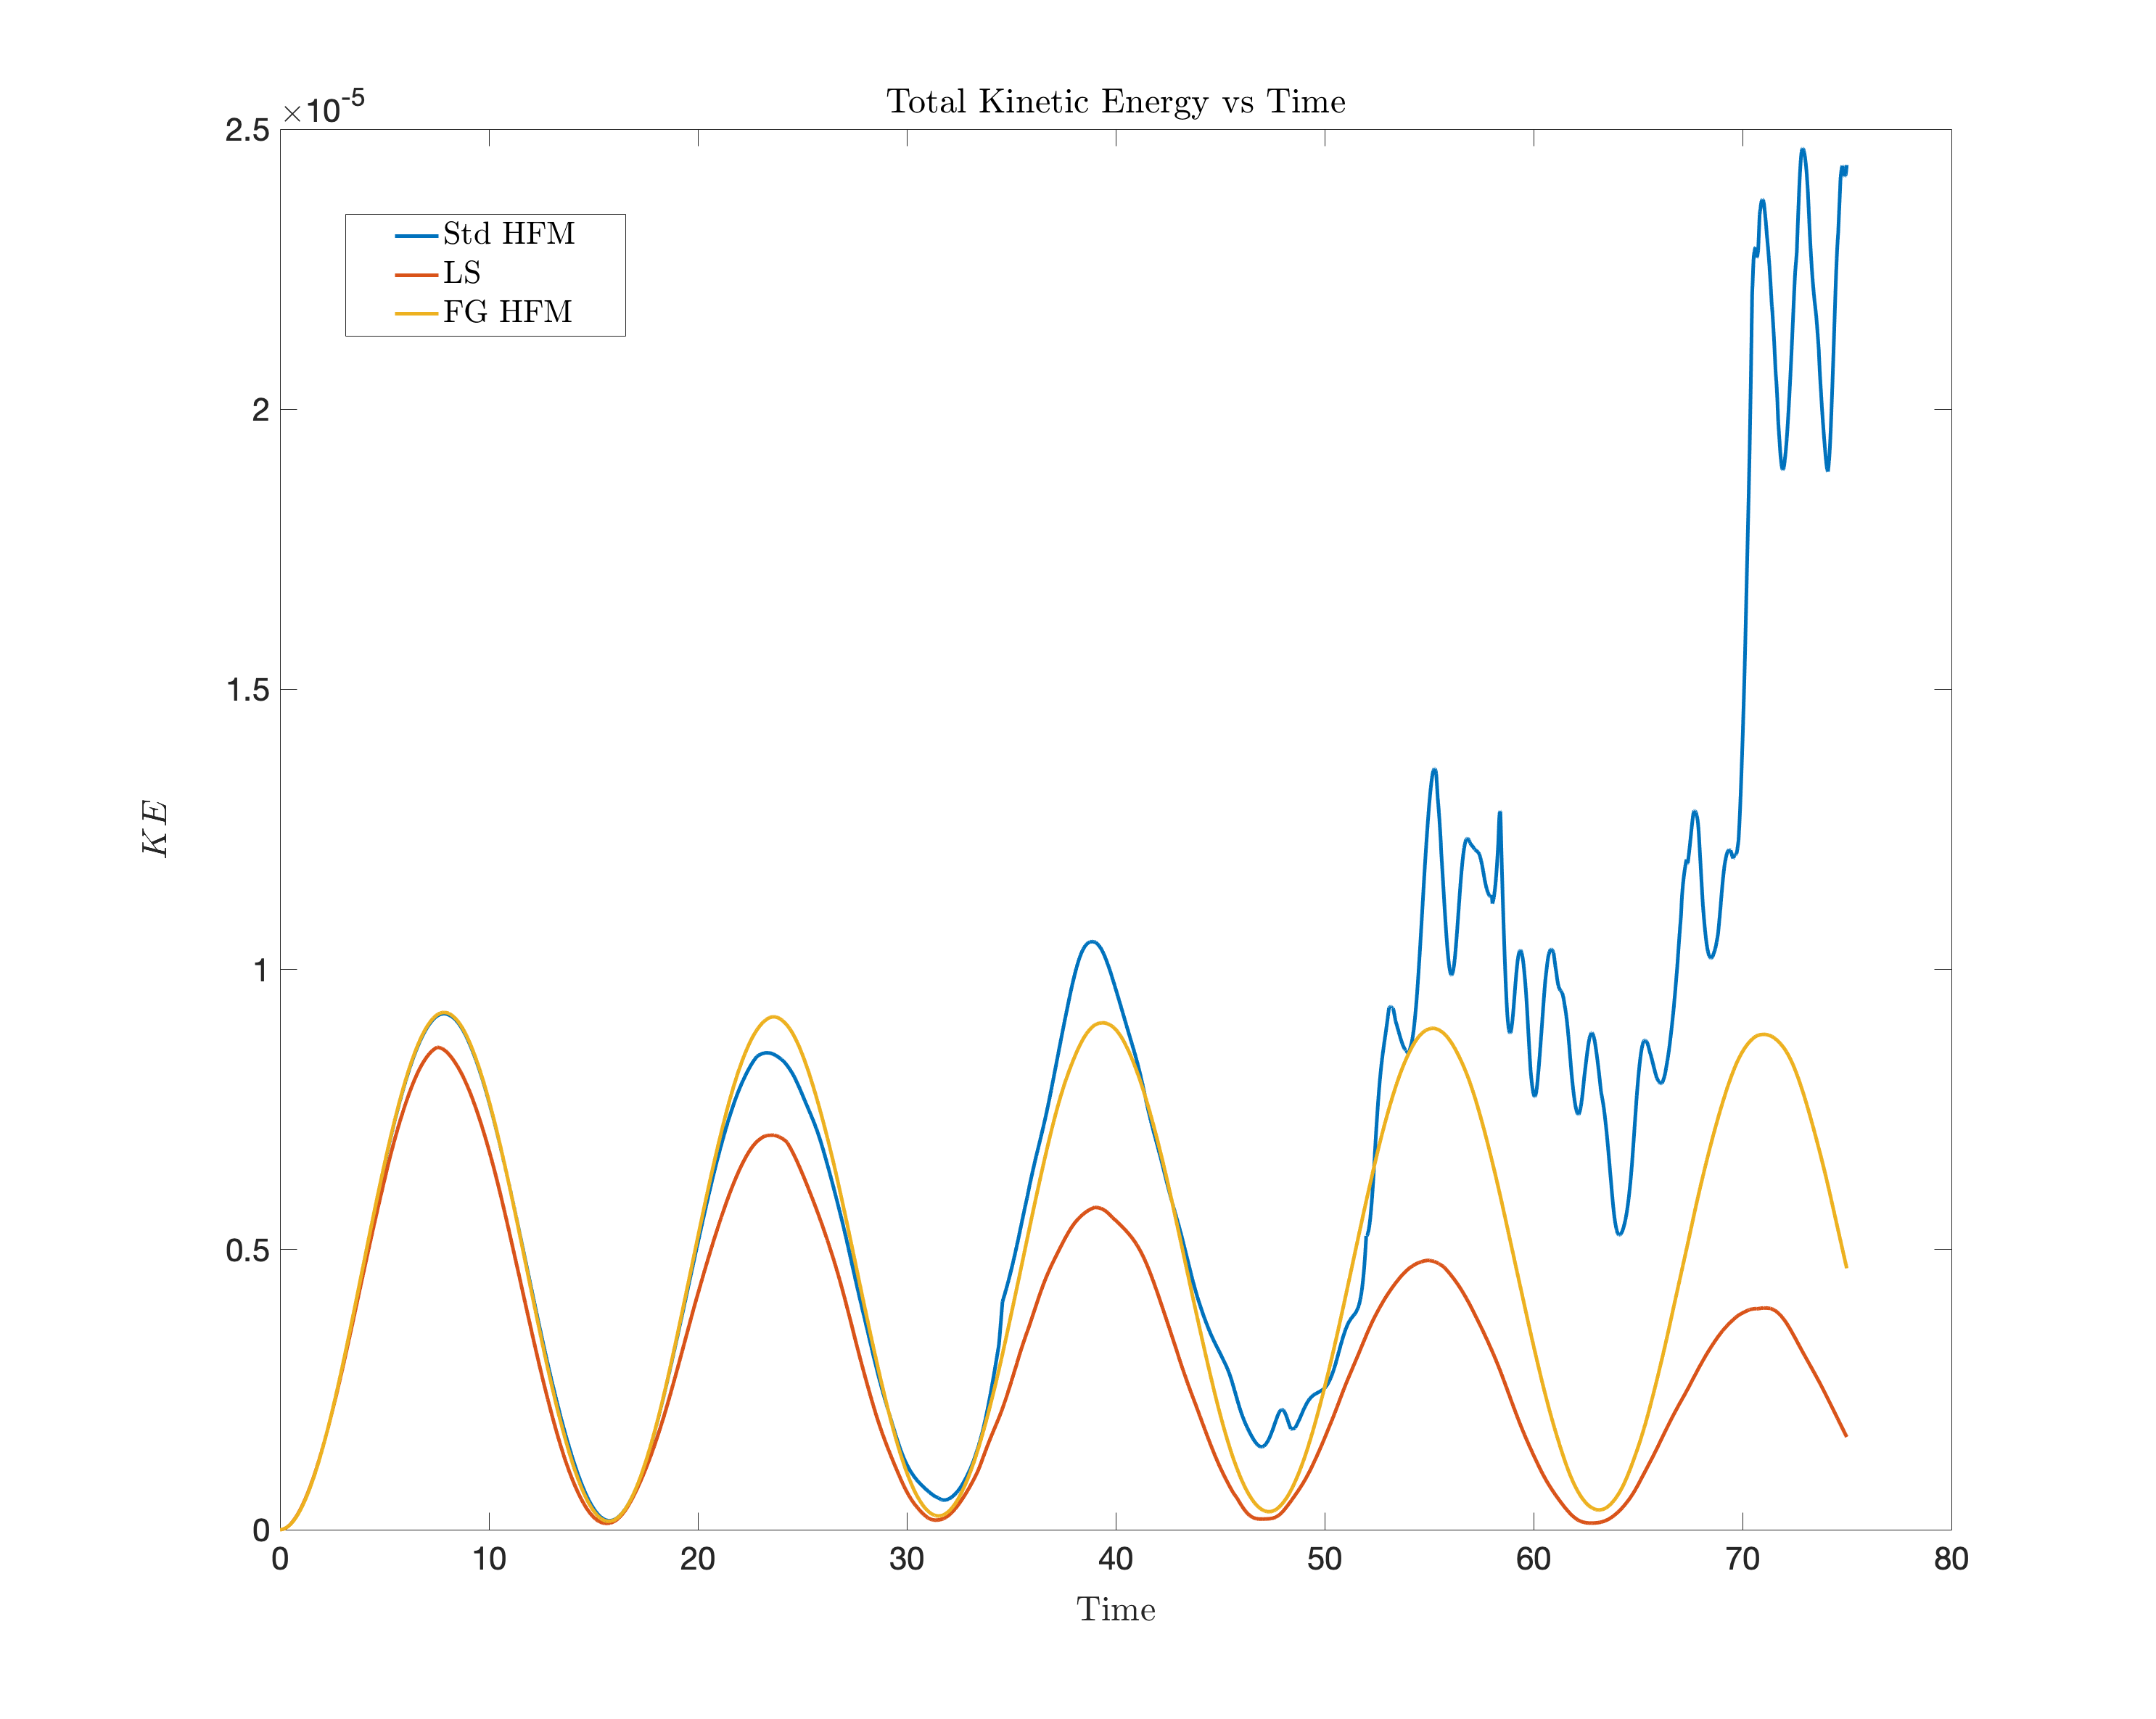
\includegraphics[width=5.0in]{figs/KEvT}
	\caption{Kinetic Energy with Time \hl{THIS IS NOT THE CORRECT FIGURE}}
	\label{fig:acesKE}
\end{figure}

 Alternatively, Figure \ref{fig:stdKE} shows the result of the same test case ran with a standard, coarse grid, curvature estimation scheme. 

\begin{figure}[htbp]
	\centering
	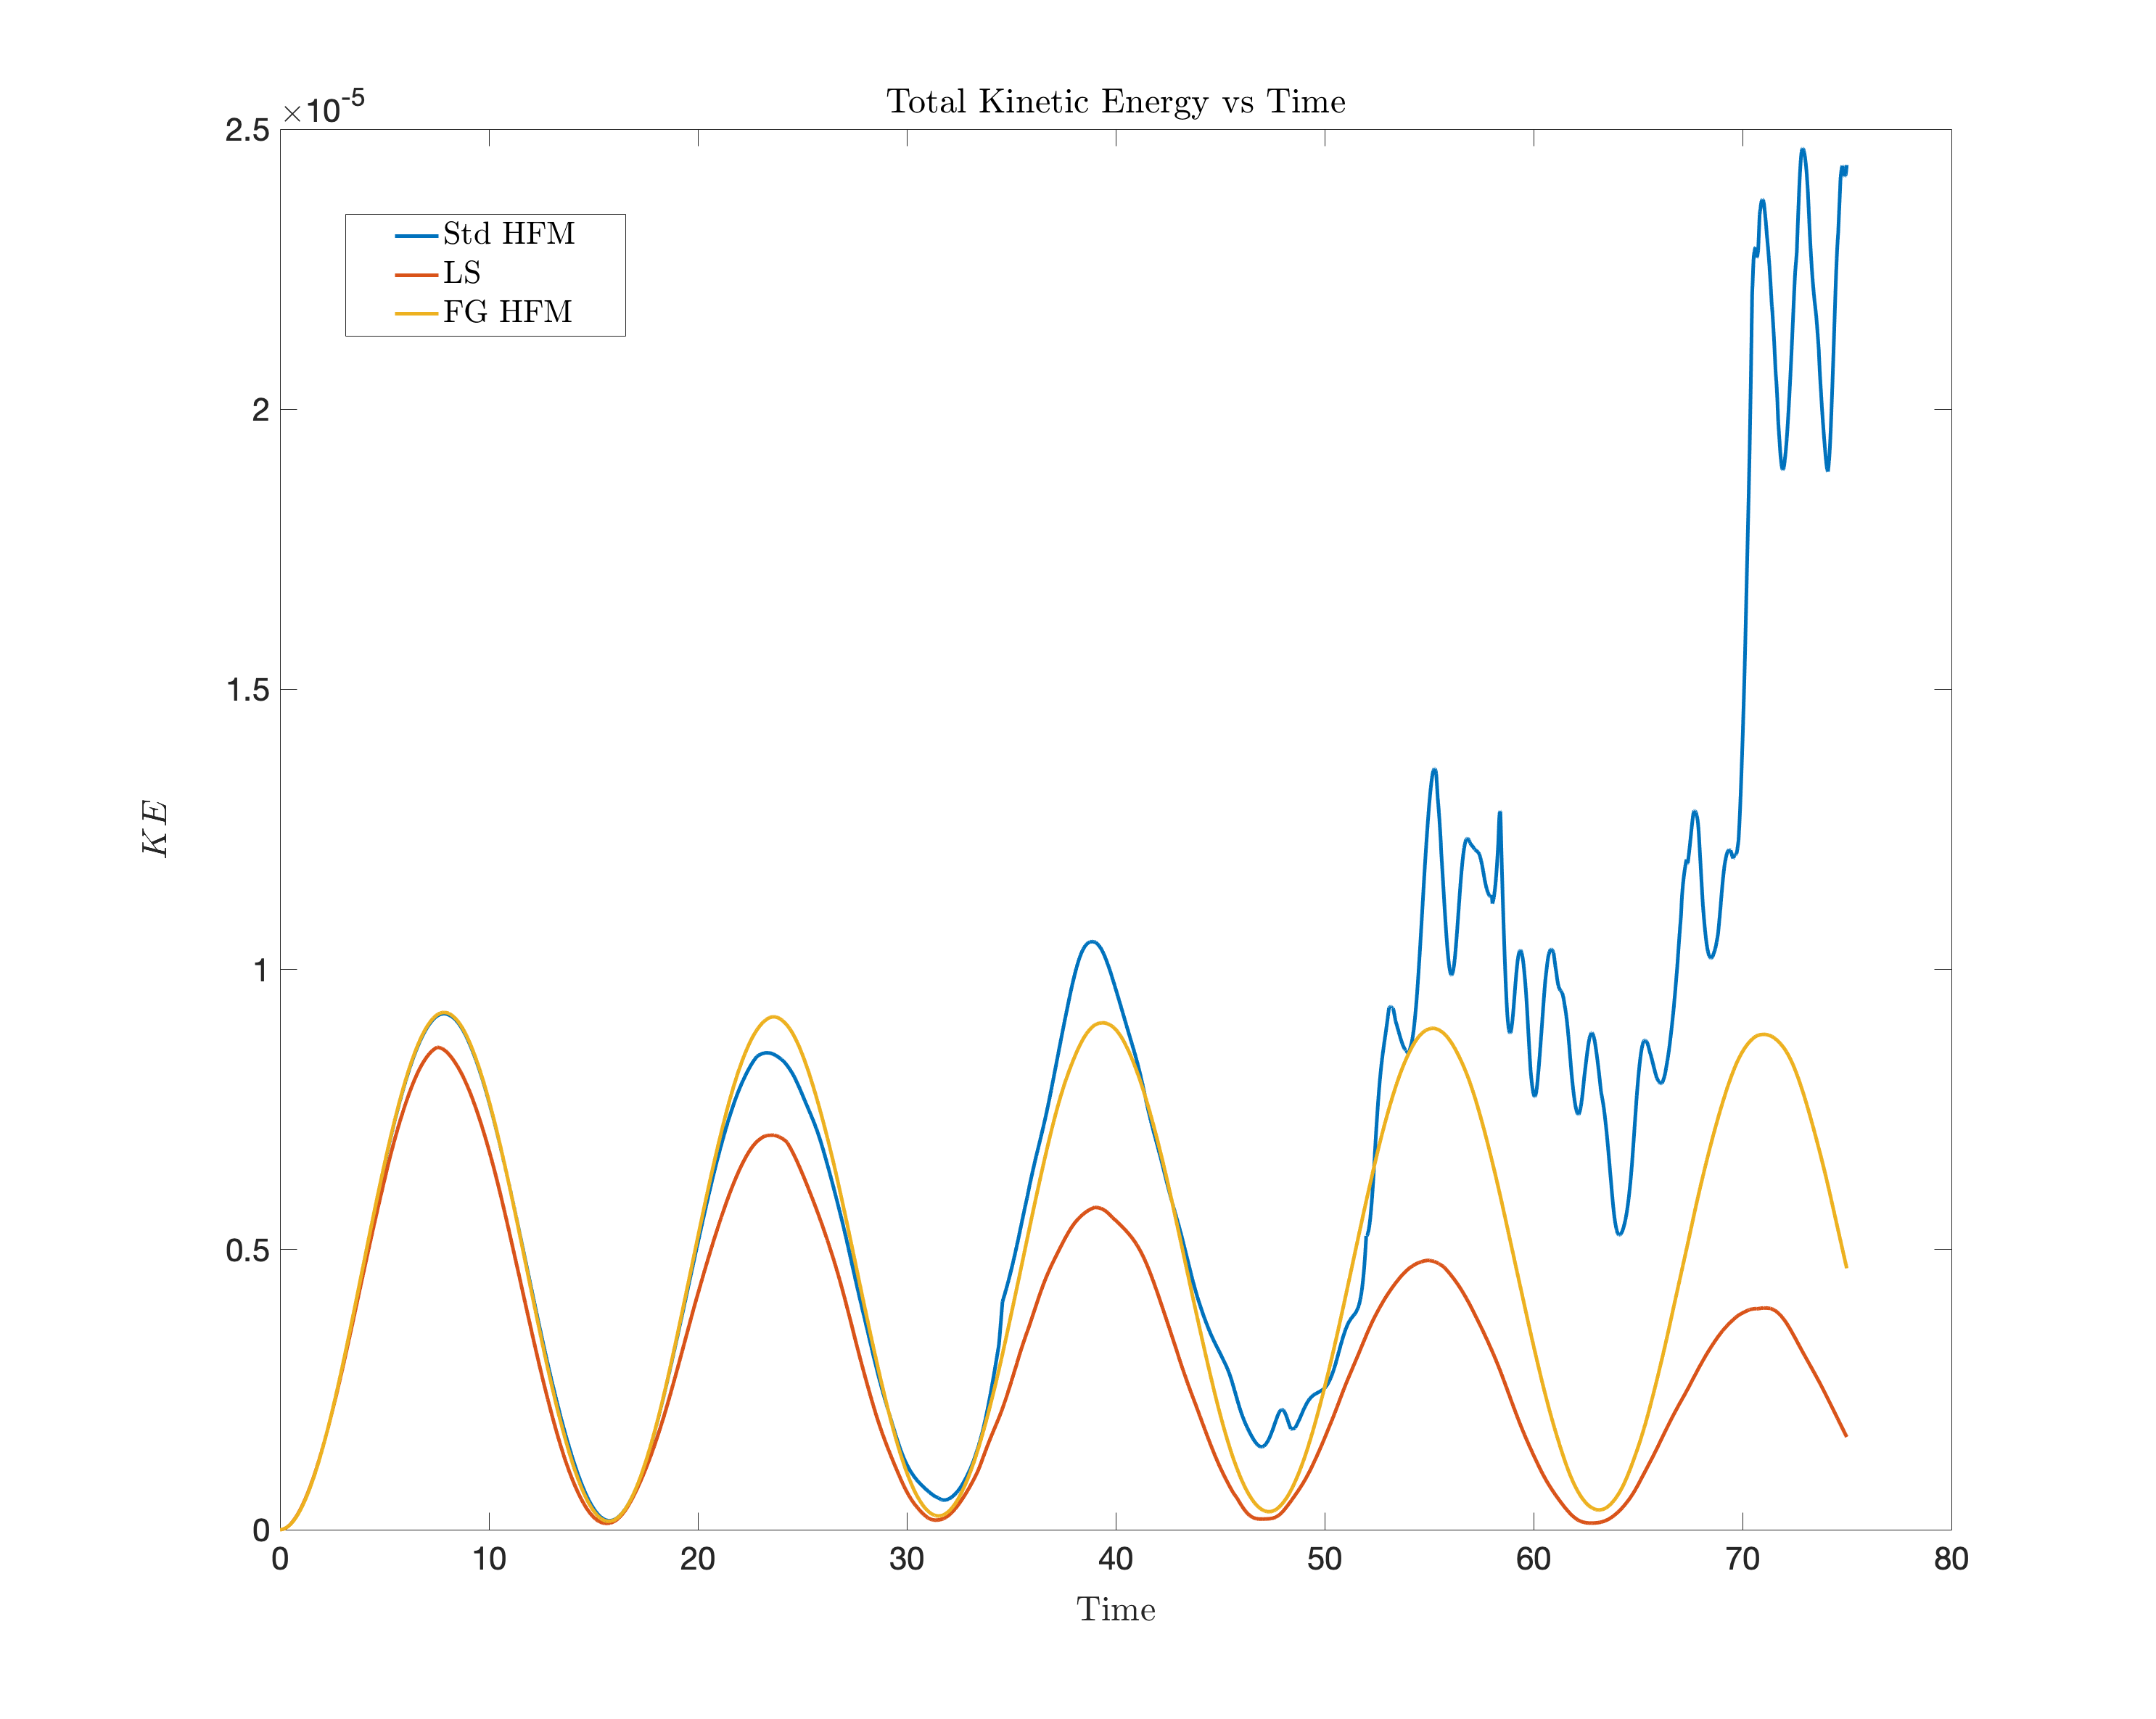
\includegraphics[width=5.0in]{figs/KEvT}
	\caption{Kinetic Energy with Time \hl{THIS IS NOT THE CORRECT FIGURE}}
	\label{fig:stdKE}
\end{figure}














































